\chapter{Empirical Evaluation}

\section{Experiment Setup}
\subsection{Experimental Subjects}
The experimental subjects used in the study is consisted of three student-developed projects that use PHP as their back-end language.

\subsection{Tools Used in Evaluation}
We evaluate the effectiveness of our interface discovery mechanism by comparing the number and quality of interfaces that it generates with the interfaces extracted by web crawlers. The web crawler tool that we used is OpenWebSpider, an open-sourced framework for crawling/spidering websites. For each interface output, we check if any of the HTTP requests in this output is processed in the back-end program.

We evaluate the effectiveness of our test request generation mechanism by comparing it against naive random test case generation. For each HTTP request, a set of possible values is generated for all of the fields in this request, creating a set of test HTTP requests, which are then sent to the server. The final code coverage of the back-end PHP code is recorded.

\section{Results}

%example%
\subsection{Email Sender}
A simple PHP program that processes a form which contains 4 input fields and sends an email according to the information supplied in the form. 

Form Inputs
\begin{itemize}
\item first\_name (required)
\item last\_name (required)
\item email (required)
\item telephone (optional)
\end{itemize}
All required fields are checked against a regular expression. The only optional field (telephone) is not checked against any regex or string variables.

Our penetration testing tool successfully identified all the fields (required and optional). It generated test cases for all the required variables from the given regex expression. For the "telephone" field, which is optional, our testing tool did not infer any information from static analysis, therefore would be producing random strings for this field during testing.

Code coverage achieved: 82.92\%

Code coverage by random generator: 60.98\%

%example%
\subsection{Fancy Hotel (CS4400 Class Project)}
A web application powered by PHP and MySQL that serves as an online room reservation system for a non-existing hotel.

\subsubsection{User Login}
Form Inputs
\begin{itemize}
\item username (string)
\item password (string)
\end{itemize}

Our penetration testing tool successfully identified both username and password fields in the interface. Since the application does not compare username and password to specific patterns or values, our static analysis did not infer possible value information for these fields. 

However, the analyzer identified session information created during login, which could potentially make subsequent penetration testing more thorough by exploiting user sessions.

In addition, the user login program can be redirected to three different URLs once login information is validated. Since these URLs are not exposed to the front-end HTML, they were not identified by web crawler. However, by performing static analysis on the source code, our penetration testing tool was able to discover all three of them.

\subsubsection{User Registration}
Form Inputs
\begin{itemize}
\item username (string)
\item password (string)
\item confirmed\_password (string)
\item email (string)
\end{itemize}

Our penetration tool successfully identified all request (or interface) parameters and their names (usn, psw, con\_pwd, email). It identified the regular expression that was used to check valid email and username in the program and used this information to construct test cases for the email and username fields.

Code coverage achieved: 91.67\%

Code coverage by random generator: 66.67\%

\subsubsection{Room Search}
Form Inputs
\begin{itemize}
  \item start\_date (string)
  \item end\_date (string)
  \item location (string)
\end{itemize}

Note
\begin{itemize}
\item start\_date must be greater than 2015-08-01;
\item start\_date cannot be greater than end\_date;
\item start\_date cannot be smaller than today’s date (2015-08-31);
\item end\_date must be smaller than 2016-01-31;
\end{itemize}

Our penetration tester successfully identified all the required fields as well as the session information not exposed by the interface itself. Furthermore, static analysis has inferred key information about both start\_date and end\_date. For start\_date, output test cases include "2015\-08\-31" and "2015\-08\-01"; for end\_date, output test cases include "2016\-01\-31". 

Code coverage achieved: 95.23\%

Code coverage by random generator: 85.71\%

%example%
\subsection{Paycheck Calculator}
A basic PHP web application that takes in one input (salary) and shows how much tax should be deduced.

Form Inputs
\begin{itemize}
  \item salary (integer)
\end{itemize}

Our penetration tool successfully identified the interface. Static analysis generated all possible numeric values that are used, either directly or indirectly, to compare with the interface input variable in the program.

Code coverage achieved: 85.37\%

Code coverage by random generator: 82.92\%

\begin{figure}
\begin{minipage}{\textwidth}
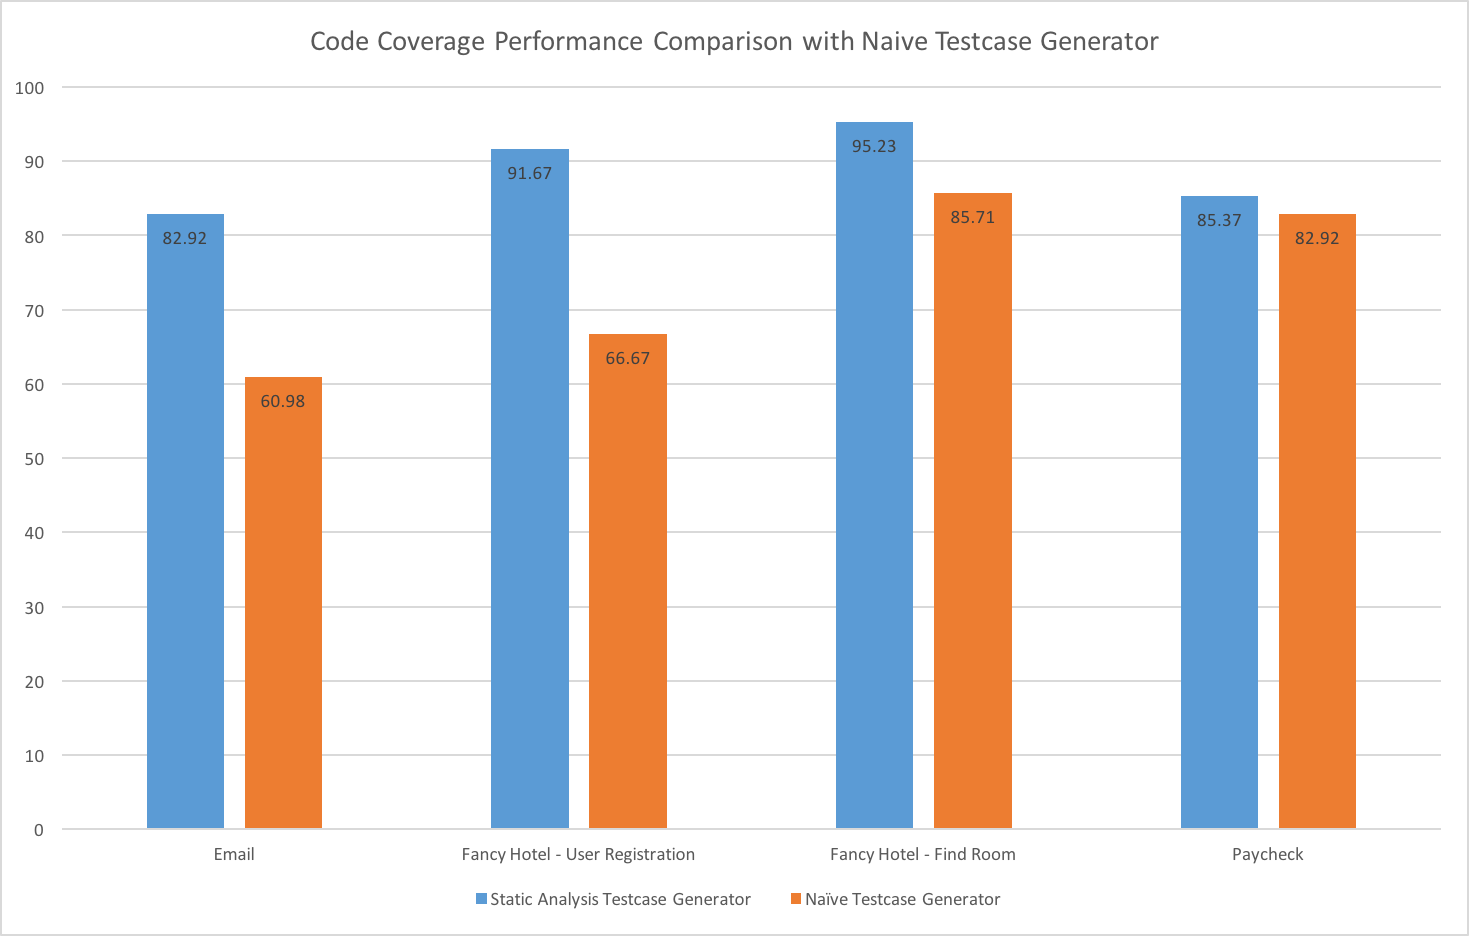
\includegraphics[width=\textwidth]{figures/result.png}
\caption{Code Coverage Performance Comparison with Naive Testcase Generator}
\label{fig:result}
\end{minipage}
\end{figure}

